\chapter{\xlabel{pol2_dr_running}POL-2 Data Reduction -- Running
  pol2map}
\label{sec:rundr}

The previous chapter, \cref{Chapter}{sec:dr}{POL-2 Data Reduction --
  The Theory}, described how \pol2map\ produces I, Q and U maps from raw
POL-2 data.  It showed that this reduction process -- which uses
\pol2map\ -- comprises three steps.

As with the other Python scripts in \SMURF, it is possible to get more
information about the available parameters by running either:
\begin{terminalv}
% pol2map --help
\end{terminalv}
or the
\begin{terminalv}
% smurfhelp pol2map
\end{terminalv}
command.

\section{\xlabel{how-pol2map}How to use pol2map}

Before running \pol2map\ directly, it is necessary to ensure that
the \starlink\ environment has been initialised and the \smurf\
package started (see \cref{Section}{sec:starinit}{Initialising
  Starlink} and \cref{Section}{sec:packinit}{KAPPA and SMURF for data
  processing}).

This chapter describes how to run \pol2map\ firstly to produce an
initial I map and then again to produce the final I, Q, U maps and
vector catalogue as described in Section~\ref{sec:how-step1}.

To run \pol2map\, values should normally be supplied for the following
command-line parameters\footnote{Note the distinction between
  ``command-line parameters'' that are supplied on the
  \pol2map\ command line, and ``configuration parameters'' that
  are specified within a configuration file. Values for all
  \emph{configuration} parameters are obtained using a single
  \emph{command-line} parameter called \param{CONFIG}.}, in order to
  produce the initial intensity image. Note that if a parameter description ends
  with a value in square brackets, it is the default value that will be used for
the parameter if no value is supplied on the command line.

\begin{aligndesc}
\item[\texttt{IN}] A list of input NDFs containing raw POL-2 data.
  There are many ways in which the list of files can be supplied, as
  described in the ``\xref{Specifying Groups of
    Objects}{sun95}{se_groups}'' section of \xref{SUN/95}{sun95}{}. The
  easiest of these is to create a simple text file containing the names of the
  raw data files (one per line), and then supply the name of the
  text file, preceded by an up-caret character (\,\texttt{\^{}}\,), as
  the value for parameter \param{IN}. Note that the specified names of the raw
  data files can contain wildcards such as ``$*$'' and ``?''.

\item[\texttt{IOUT}] The name of the NDF in which to store the
  total intensity (I) map (in pW) incorporating all supplied observations.
  The supplied file name should either have a file type of
  \texttt{.sdf}, or no file type at all (in which case
  \texttt{.sdf} will be appended to the supplied value). Any existing
  file with the same name will be overwritten.

\item[\texttt{QOUT}] The output NDF in which to return the Q map
  incorporating all supplied observations. This will be in units of
  pW. Null (\texttt{!}) should be supplied if no Q map is required.

\item[\texttt{UOUT}] The output NDF in which to return the U map
  incorporating all supplied observations. This will be in units of
  pW. Null (\texttt{!}) should be supplied if no U map is required.

\item[\texttt{MAPDIR}] The name of the directory in which to place the Q,
  U and I maps made from each individual observation supplied via
  \param{IN}, before co-adding them. If null (\texttt{!}) is supplied, the new
  maps are placed in the same temporary directory (chosen automatically)
  as all the other intermediate files, and so will be deleted when the script
  exits (unless the parameter \param{RETAIN} is set to be \texttt{TRUE}). Note
  that these maps are always in units of pW. Each one will contain FITS
  headers specifying the pointing corrections needed to align the map with
  the reference map. [\texttt{!}]

\item[\texttt{QUDIR}] The name of a directory in which to place the Q, U
  and I time series generated by \SMURF\ \task{calcqu}, prior to generating
  maps from them. If null (\texttt{!}) is supplied, they are placed in the same
  temporary directory as all the other intermediate files, and so will
  be deleted when the script exits (unless the parameter \param{RETAIN} is
  set to be \texttt{TRUE}). [\texttt{!}]
\end{aligndesc}

Some additional command-line parameters are required when \pol2map\ is
used for the second time -- as discussed in Section~\ref{sec:how-step23}
-- to produce the final I, Q, U maps and vector catalogue\footnote{This
second usage of \pol2map\ includes both ``Run 2'' and ``Run 3'' in
Figure~\ref{fig:pol2drflow}.}.

\begin{aligndesc}

\item[\texttt{CAT}] The output FITS vector catalogue. No catalogue is
  created if null (!) is supplied. Note that, by default, the Q, U and
  I$_{\textnormal{p}}$ values in this catalogue will be in units of mJy/beam. [!]

\item[\texttt{MASK}] Specifies the type of masking to be used within
  \makemap\ (the same type of masking is used to create all three maps --
  I, Q and U).

\item[\texttt{MASKOUT1}] If a non-null value is supplied for \param{MASKOUT1},
  it specifies the NDF in which to store the AST mask created from the NDF
  specified by Parameter \param{MASK}. Only used if an NDF is supplied for
  Parameter \param{MASK}. [!]

\item[\texttt{MASKOUT2}] If a non-null value is supplied for \param{MASKOUT2},
  it specifies the NDF in which to store the PCA mask created from the NDF
  specified by Parameter \param{MASK}. Only used if an NDF is supplied for
  Parameter \param{MASK}. [!]

\item[\texttt{IPREF}] The total intensity map to be used for IP
  correction. The map must be in units of pW. If the same value is
  supplied for both \param{IOUT} and \param{IPREF}, the output I
  map will be used for IP correction. [\texttt{!}]

\item[\texttt{DEBIAS}] \texttt{TRUE} if a correction for statistical bias is to
  be made to percentage polarisation and polarised intensity in the
  output vector catalogue specified by the parameter \param{CAT}. [\texttt{FALSE}]
\end{aligndesc}

The \pol2map\ command provides many other parameters that may be used to
modify its behaviour in various ways. To see a full list, type

\begin{terminalv}
% pol2map --help
\end{terminalv}


\section{\xlabel{how-step1}pol2map -- producing the initial I map}
\label{sec:how-step1}

As discussed in \cref{Chapter}{sec:dr}{POL-2 Data Reduction -- The
  Theory},\pol2map\ must first be run on the raw data to produce an
initial I map.  In this first step:

\begin{terminalv}
% pol2map in=^myfiles.list iout=iauto qout=! uout=! mapdir=maps qudir=qudata
\end{terminalv}

The file \texttt{myfiles.lis} contains a list of the raw data
files to be included in the map, and could (for instance) look like
this:

\begin{terminalv}
% cat myfiles.lis
/jcmtdata/raw/scuba2/s8a/20160125/00043/*
/jcmtdata/raw/scuba2/s8b/20160125/00043/*
/jcmtdata/raw/scuba2/s8c/20160125/00043/*
/jcmtdata/raw/scuba2/s8d/20160125/00043/*
\end{terminalv}

This uses all available data from all four 850\,$\mu$m sub-arrays, for
Observation 43 taken on 25th January 2016\footnote{The input files
  should all be for a single waveband from one or more POL-2
  observations. Users should not mix files from different wavebands and/or
  astronomical regions.}. In addition, the data used in this example
also come from Observations 56 and 59 taken on January 11th 2016 (UT).

\begin{tip}
  An up-caret ( $ \hat{} $ ) is required any time the user is reading in
  a group text file in Starlink. For the map-maker, this includes the
  configuration file (a group of configuration parameters) and the
  list of input files (a group of NDFs \emph{e.g.} \texttt{in= $
    \hat{} $ myfiles.lis}).

  Note that the \pol2map\ script also invokes the \ \smurf\
  \xref{pol2check}{sun258}{POL2CHECK} command, in order to 
  first ensure that the input files are actually POL-2 files.
\end{tip}

Note that \texttt{qout} and \texttt{uout} are set to null values, as no
Q or U maps are required to be produced during this initial step 1
reduction stage.

The following shows the output from running this initial \pol2map\
command.

\begin{terminalv}
Logging to file pol2map.log
Calculating Q, U and I time streams from raw analysed intensity data...
   1/3: Processing 116 raw data files from observation 20160125_00043 ...
   2/3: Processing 116 raw data files from observation 20160112_00059 ...
   3/3: Processing 116 raw data files from observation 20160112_00056 ...

>>>>   Making I map from 20160125_00043_0003...

>>>>   Making I map from 20160112_00056_0003...

>>>>   Making I map from 20160112_00059_0003...

Co-adding I maps from all observations:

20160125_00043_0003: Storing pointing corrections of (0.0,0.0) arc-seconds
for future use

20160112_00056_0003: Storing pointing corrections of (1.9,2.8) arc-seconds
for future use

20160112_00059_0003: Storing pointing corrections of (2.1,2.4) arc-seconds
for future use

\end{terminalv}

The files and folders produced by this reduction process are described below.

\begin{aligndesc}
\item[\file{pol2map.log}] A log file containing the output from the
  various \SMURF, \KAPPA\ and \POLPACK\ commands run as part of the \pol2map\
  command (\pol2map\ is actually a Python script that runs various other
  Starlink tasks behind the scenes in order to perform the bulk of the work).

\item[\file{qudata/}] A folder containing the I, Q and U time-series data
  for each sub array for each observation. Tthese are produced by
  \task{calcqu} (see Section~\cref{Chapter}{sec:calcqu}{CALCQU}.

\item[\file{maps/}] A folder containing the individual I maps from
  each separate observation. These will have names that end with
  \file{$\_$imap.sdf}.

\item[\file{iauto.sdf}] Output total intensity map. The included term ``auto'' is
used to indicate that it was created using an automatically generated
AST mask.

\end{aligndesc}

The output I map, \file{iauto.sdf}, can be opened and viewed with \GAIA.

\begin{figure}[t!]
\begin{center}
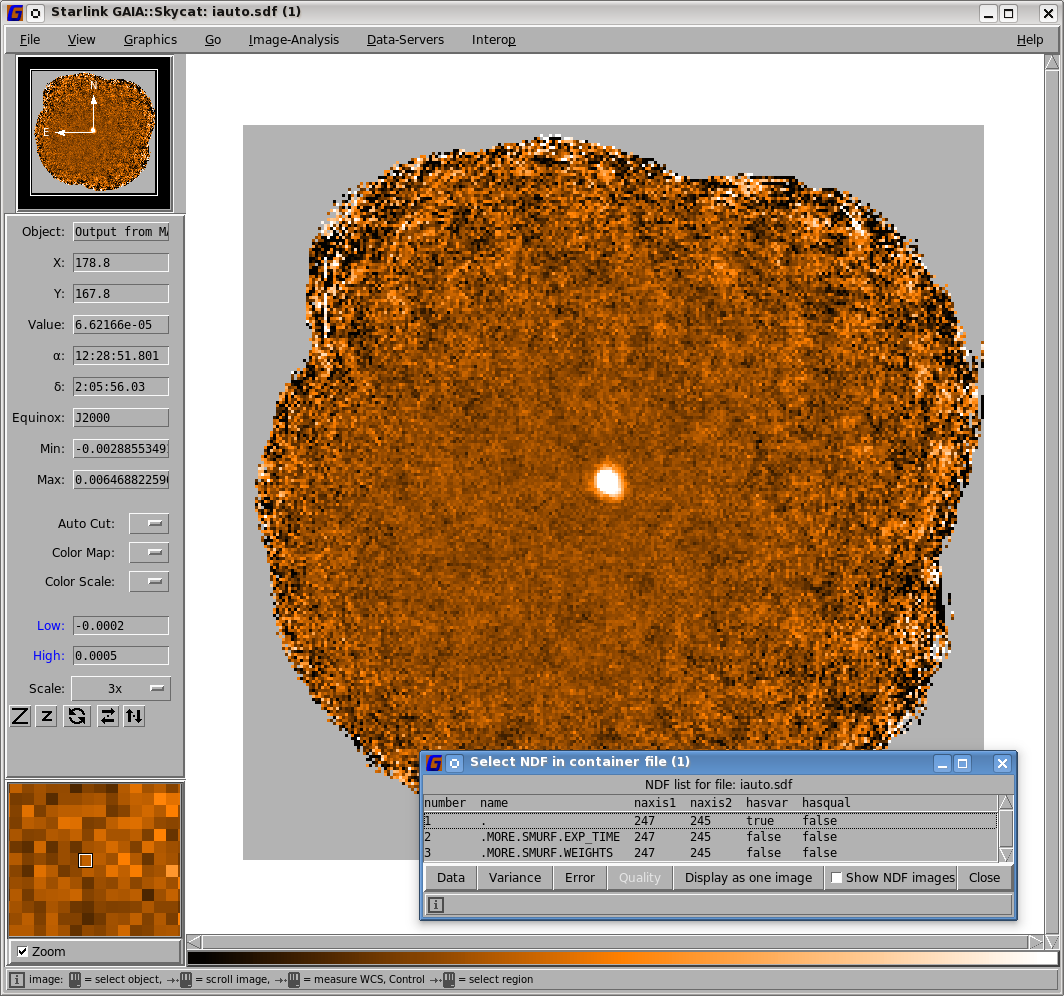
\includegraphics[width=0.8\linewidth]{sc22-gaia-view-iauto.png}
\label{fig:gaia-iauto}
\caption [I map in GAIA]{
  \small The I map, \file{iauto.sdf}, as viewed with \GAIA.
}
\end{center}
\end{figure}

The \file{maps} folder contains the individual I maps from each separate
observation:

\begin{terminalv}
20160112_00056_0003_imap.sdf  20160112_00059_0003_imap.sdf  20160125_00043_0003_imap.sdf
\end{terminalv}

and the \file{qudata} folder contains these files.

\begin{terminalv}
s8a20160112_00056_0003_IT.sdf  s8b20160112_00059_0003_IT.sdf  s8c20160125_00043_0003_IT.sdf
s8a20160112_00056_0003_QT.sdf  s8b20160112_00059_0003_QT.sdf  s8c20160125_00043_0003_QT.sdf
s8a20160112_00056_0003_UT.sdf  s8b20160112_00059_0003_UT.sdf  s8c20160125_00043_0003_UT.sdf
s8a20160112_00059_0003_IT.sdf  s8b20160125_00043_0003_IT.sdf  s8d20160112_00056_0003_IT.sdf
s8a20160112_00059_0003_QT.sdf  s8b20160125_00043_0003_QT.sdf  s8d20160112_00056_0003_QT.sdf
s8a20160112_00059_0003_UT.sdf  s8b20160125_00043_0003_UT.sdf  s8d20160112_00056_0003_UT.sdf
s8a20160125_00043_0003_IT.sdf  s8c20160112_00056_0003_IT.sdf  s8d20160112_00059_0003_IT.sdf
s8a20160125_00043_0003_QT.sdf  s8c20160112_00056_0003_QT.sdf  s8d20160112_00059_0003_QT.sdf
s8a20160125_00043_0003_UT.sdf  s8c20160112_00056_0003_UT.sdf  s8d20160112_00059_0003_UT.sdf
s8b20160112_00056_0003_IT.sdf  s8c20160112_00059_0003_IT.sdf  s8d20160125_00043_0003_IT.sdf
s8b20160112_00056_0003_QT.sdf  s8c20160112_00059_0003_QT.sdf  s8d20160125_00043_0003_QT.sdf
s8b20160112_00056_0003_UT.sdf  s8c20160112_00059_0003_UT.sdf  s8d20160125_00043_0003_UT.sdf
\end{terminalv}


\section{\xlabel{how-step23}pol2map -- producing the I, Q, U maps and catalogue}
\label{sec:how-step23}

As discussed in \cref{Chapter}{sec:dr}{POL-2 Data Reduction -- The
  Theory}, the I map output from the initial run of \pol2map\ is used to
derive the final I, Q and U maps. If requested, a vector catalogue is
also produced.

The second and third steps of the POL-2 data reduction process can be
run via a single command.

\begin{terminalv}
% pol2map in=qudata/\* iout=iext qout=qext uout=uext mapdir=maps mask=iauto \
          maskout1=astmask maskout2=pcamask ipref=iext cat=mycat debias=yes
\end{terminalv}

The following shows the output from running this second \pol2map\
command. First, \pol2map\ produces new I maps for each map, correcting
the position using the correction stored in the old I
map\footnote{This correction is found by aligning the old I map with the
\file{iauto.sdf} map.}, and then co-adds all the observations.

\begin{terminalv}
Logging to file pol2map.log
(existing file pol2map.log moved to pol2map.log.1)

Masking will be based on SNR values in 'iauto'.

>>>>   Making I map from 20160112_00056_0003...

   Using pre-calculated pointing corrections of (1.9,2.8) arc-seconds

>>>>   Making I map from 20160125_00043_0003...

   Using pre-calculated pointing corrections of (0.0,0.0) arc-seconds

>>>>   Making I map from 20160112_00059_0003...

   Using pre-calculated pointing corrections of (2.1,2.4) arc-seconds
Coadding I maps from all observations:
\end{terminalv}

As \pol2map\ continues, the Q and U maps are produced, again with
pointing corrections. This is followed by the creation of the output
vector catalogue.

\begin{terminalv}
>>>>   Making Q map from 20160112_00056_0003...

   Using pre-calculated pointing corrections of (1.9,2.8) arc-seconds

>>>>   Making Q map from 20160125_00043_0003...

   Using pre-calculated pointing corrections of (0.0,0.0) arc-seconds

>>>>   Making Q map from 20160112_00059_0003...

   Using pre-calculated pointing corrections of (2.1,2.4) arc-seconds
Coadding Q maps from all observations:

>>>>   Making U map from 20160112_00056_0003...

   Using pre-calculated pointing corrections of (1.9,2.8) arc-seconds

>>>>   Making U map from 20160125_00043_0003...

   Using pre-calculated pointing corrections of (0.0,0.0) arc-seconds

>>>>   Making U map from 20160112_00059_0003...

   Using pre-calculated pointing corrections of (2.1,2.4) arc-seconds
Coadding U maps from all observations:
Creating the output catalogue: 'mycat'...

45604 vectors written to the output catalogue.
\end{terminalv}


The output of this final run of \pol2map\ is as follows.

\begin{aligndesc}
\item[\file{pol2map.log}] A log file containing the output from the
  \pol2map\ command. Note previous log files are moved to a new name
  such as \texttt{pol2map.log.1}.

\item[\file{astmask.sdf}] The AST mask used in the creation
  of the final I, Q and U maps.

\item[\file{pcamask.sdf}] The PCA mask used in the creation of the
  final I, Q and U maps.

\item[\file{iext.sdf}] The total intensity image, created using the
  external AST and PCA masks described above.

\item[\file{qext.sdf}] The Q map (\emph{i.e} the intensity of the radiation
  linearly polarised in the direction parallel or perpendicular to the
  reference plane), created using an external AST and PCA mask.

\item[\file{maps/}] A folder containing the individual I, Q and U
  maps from each separate observation. These will have names that end with
  \file{$\_$Imap.sdf}, \file{$\_$Qmap.sdf} or \file{$\_$Umap.sdf}.

\item[\file{uext.sdf}] The U map (\emph{i.e.} the intensity of the radiation
  linearly polarised in the direction $\pm45^{\circ }$ to the reference plane).

\item[\file{mycat.FIT}] The output vector catalogue containing a
  range of values derived by \pol2map\ for each pixel contained within
  the I map.

\end{aligndesc}


\begin{figure}[t!]
\begin{center}
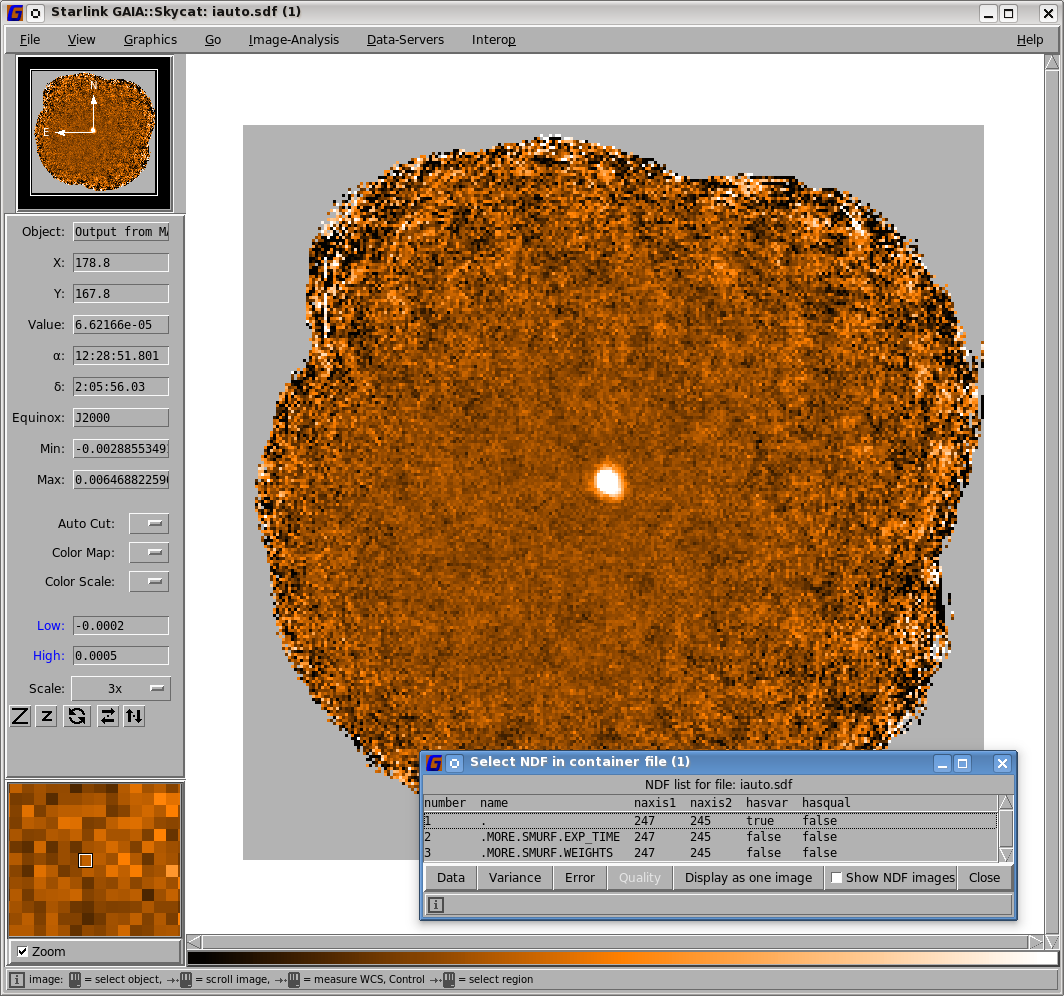
\includegraphics[width=0.46\linewidth]{sc22-gaia-view-iauto.png}
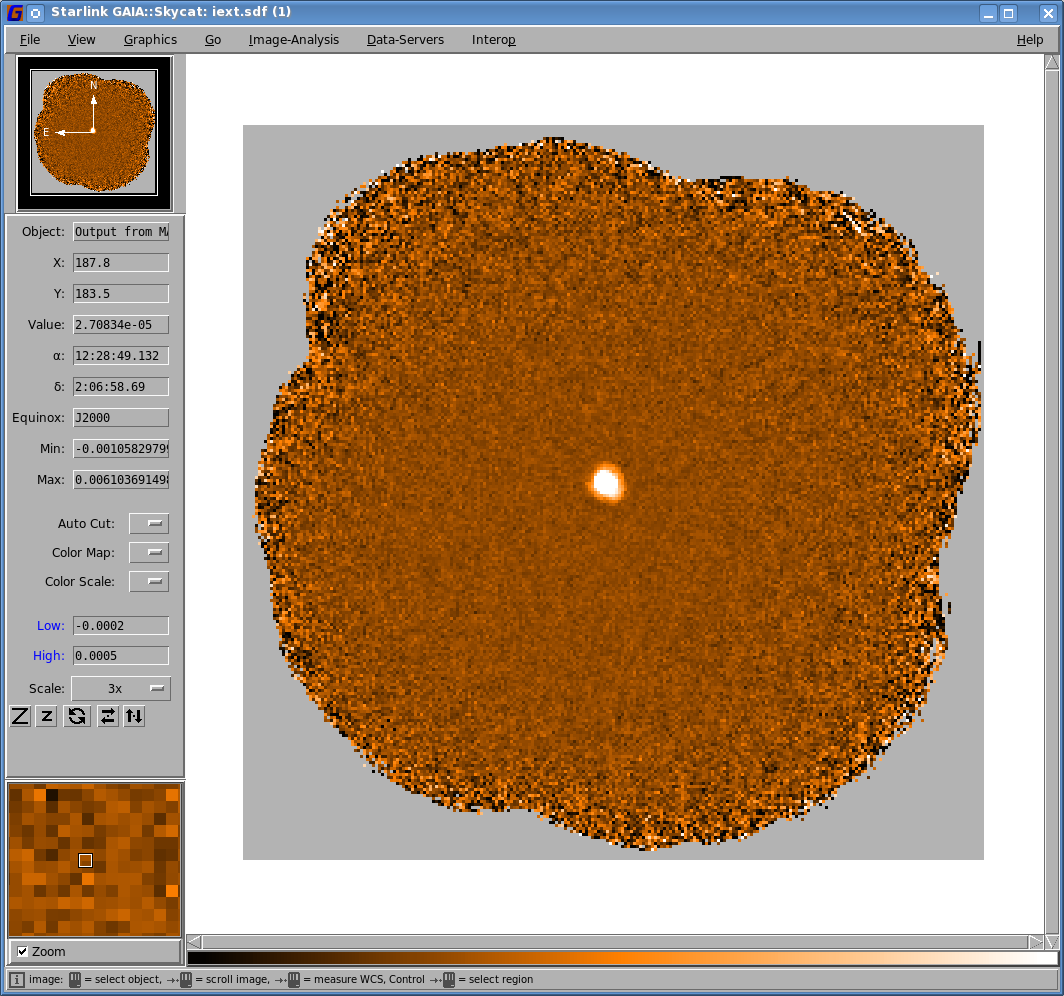
\includegraphics[width=0.46\linewidth]{sc22-gaia-view-iext.png}
\label{fig:gaia-iext}
\caption [Final I map in GAIA]{
  \small Left: I map, \file{iauto}, as produced by the automask on the first pass
         of \pol2map\. Right: Final I map, \file{iext}, as viewed in \GAIA.
         The flatter background is due to the increase in \param{pca.pcathresh}.
}
\end{center}
\end{figure}


\begin{figure}[t!]
\begin{center}
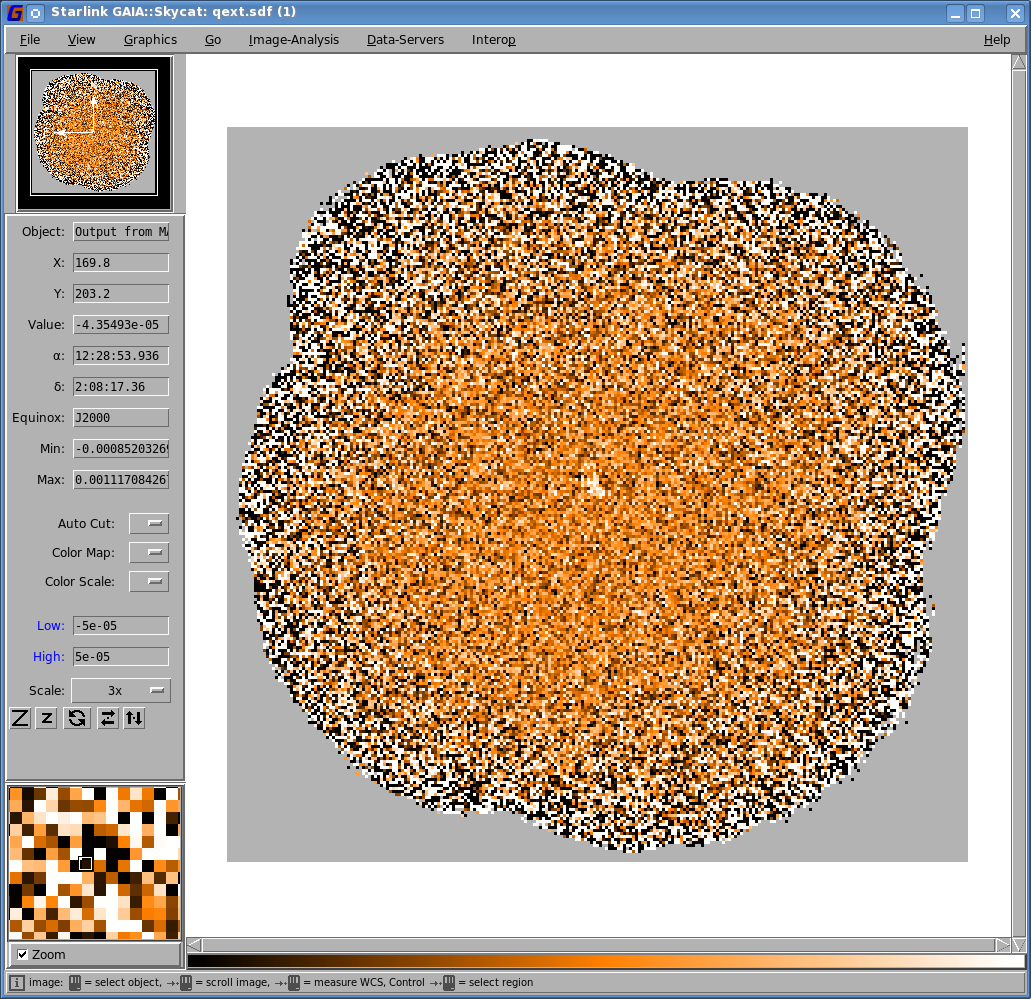
\includegraphics[width=0.46\linewidth]{sc22-gaia-view-qext.png}
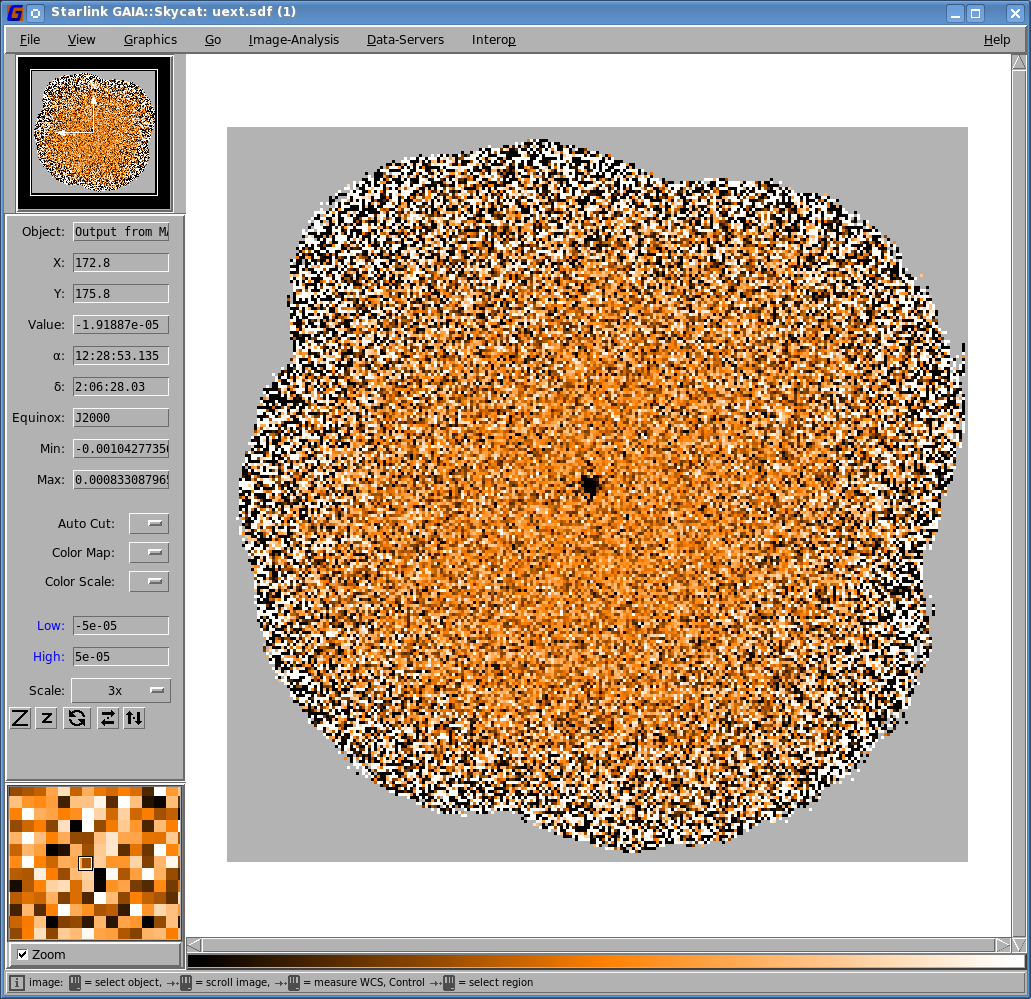
\includegraphics[width=0.46\linewidth]{sc22-gaia-view-uext.png}
\label{fig:gaia-qext-uext}
\caption [Q and U maps in GAIA]{
  \small Left: Q map, \file{qext.sdf}. Right: U map \file{uext.sdf}, as viewed with \GAIA.
}
\end{center}
\end{figure}



The maps folder now contains individual Q and U maps alongside the
existing I maps listed below.

\begin{terminalv}
20160112_00056_0003_Imap.sdf  20160112_00059_0003_Imap.sdf  20160125_00043_0003_Imap.sdf
20160112_00056_0003_Qmap.sdf  20160112_00059_0003_Qmap.sdf  20160125_00043_0003_Qmap.sdf
20160112_00056_0003_Umap.sdf  20160112_00059_0003_Umap.sdf  20160125_00043_0003_Umap.sdf
20160112_00056_0003_imap.sdf  20160112_00059_0003_imap.sdf  20160125_00043_0003_imap.sdf
\end{terminalv}




\section{\xlabel{vector-cat}Output vectors from pol2map}



The output vector catalogue contains a range of values derived by
\pol2map\ for each pixel contained within the I map. Intensity values and
errors in the
catalogue are expressed in units of mJy/beam.  If desired it is possible
to switch the catalogue to units of pW by using \texttt{Jy=no} on the \pol2map\
command line.  The columns are listed below.

\begin{aligndesc}
\item[\texttt{X}] Pixel coordinate at the centre of the pixel
\item[\texttt{Y}] Pixel coordinate at the centre of the pixel
\item[\texttt{RA}] RA coordinate at the centre of the pixel
\item[\texttt{Dec}] Dec coordinate at the centre of the pixel
\item[\texttt{I}] Total intensity
\item[\texttt{DI}] Error in I
\item[\texttt{Q}] Stokes Q parameter
\item[\texttt{DQ}] Error in Q
\item[\texttt{U}] Stokes U parameter
\item[\texttt{DU}] Error in U
\item[\texttt{P}] Percentage polarisation
\item[\texttt{DP}] Error in P
\item[\texttt{ANG}] Angle of polarisation
\item[\texttt{DANG}] Error in ANG
\item[\texttt{PI}] Polarised intensity (I$_{\textnormal{p}}$)
\item[\texttt{DPI}] Error in polarised intensity
\end{aligndesc}


\section{\xlabel{pol2fcf}POL-2 FCFs}
\label{sec:pol2map-fcf}

Inserting POL-2 in front of SCUBA-2 reduces the throughput to SCUBA-2.
POL-2 is not a perfect polarimeter. Its wire grid absorbs and scatters incoming
signal so the modulation amplitude is lower than for a perfect polarimeter.
In addition cross polarization and depolarization decreases the modulation
amplitude without decreasing the power in the transmitted signal. The first
type of inefficiencies can be measured by comparing normal SCUBA-2 maps with
and without the polarimeter inserted. Such observations have been done on Uranus,
Mars and Jupiter. The second type of losses can be measured with a source of know polarization.

To convert POL-2 data to astronomical units such as mJy/beam a Flux Conversion
Factor, FCF, must be applied to the data. For POL-2 the FCFs are quoted in terms of
the SCUBA-2 FCF.

At \SI{850}{\micro\metre} and \SI{450}{\micro\metre} the FCFs for POL-2
are found to be a factor of 1.35 and 1.96 times higher than the
standard SCUBA-2 FCF for \SI{850}{\micro\metre} and \SI{450}{\micro\metre}, respectively.


\section{\xlabel{tweaking}Changing pixel size in pol2map}
\label{sec:pol2map-pixelsize}

Inevitably, as with unpolarised SCUBA-2 data reduction, it will
probably be necessary for you to tweak the \pol2map\ reduction for
specific situations.

The bin size within the final vector catalogue is controlled by the
\param{BINSIZE} parameter in the \SMURF\ \pol2map\ command.

\begin{terminalv}
% pol2map binsize=12
\end{terminalv}

Changing the catalogue bin size in this way does not change the pixel
size of the maps created \pol2map\. Instead, the maps are binned up
to the requested bin size before the catalogue is created. There is
another parameter, called \param{PIXSIZE}, which controls the map pixel
size, but it is usually advisable to leave this at its default value
as the map pixel size can affect the behaviour of the iterative algorithm
used to create maps.







